% Chapter 1

\chapter{Methodology and Requirements} % Main chapter title

\label{Chapter2} % For referencing the chapter elsewhere, use \ref{Chapter1} 

%----------------------------------------------------------------------------------------

% % Define some commands to keep the formatting separated from the content 
% \newcommand{\keyword}[1]{\textbf{#1}}
% \newcommand{\tabhead}[1]{\textbf{#1}}
% \newcommand{\code}[1]{\texttt{#1}}
% \newcommand{\file}[1]{\texttt{\bfseries#1}}
% \newcommand{\option}[1]{\texttt{\itshape#1}}

%----------------------------------------------------------------------------------------

\section{Background}

As Figure \ref{fig:traditional_data_model} demonstrates, the traditional way for researchers to process data which they do not produce themselves or already possess is to first transfer the data from a remote holding source to themselves. This process is almost always the bottleneck in data processing as large data sets can take a large amount of time to retrieve. This is a growing issue and will continue to become more serious as time progresses and data sizes increase. Data processing capabilities must be made more readily available at institutions that carry large data sets to offset the amount of time wasted in transferring such data.

\begin{figure}[ht!]
\centering
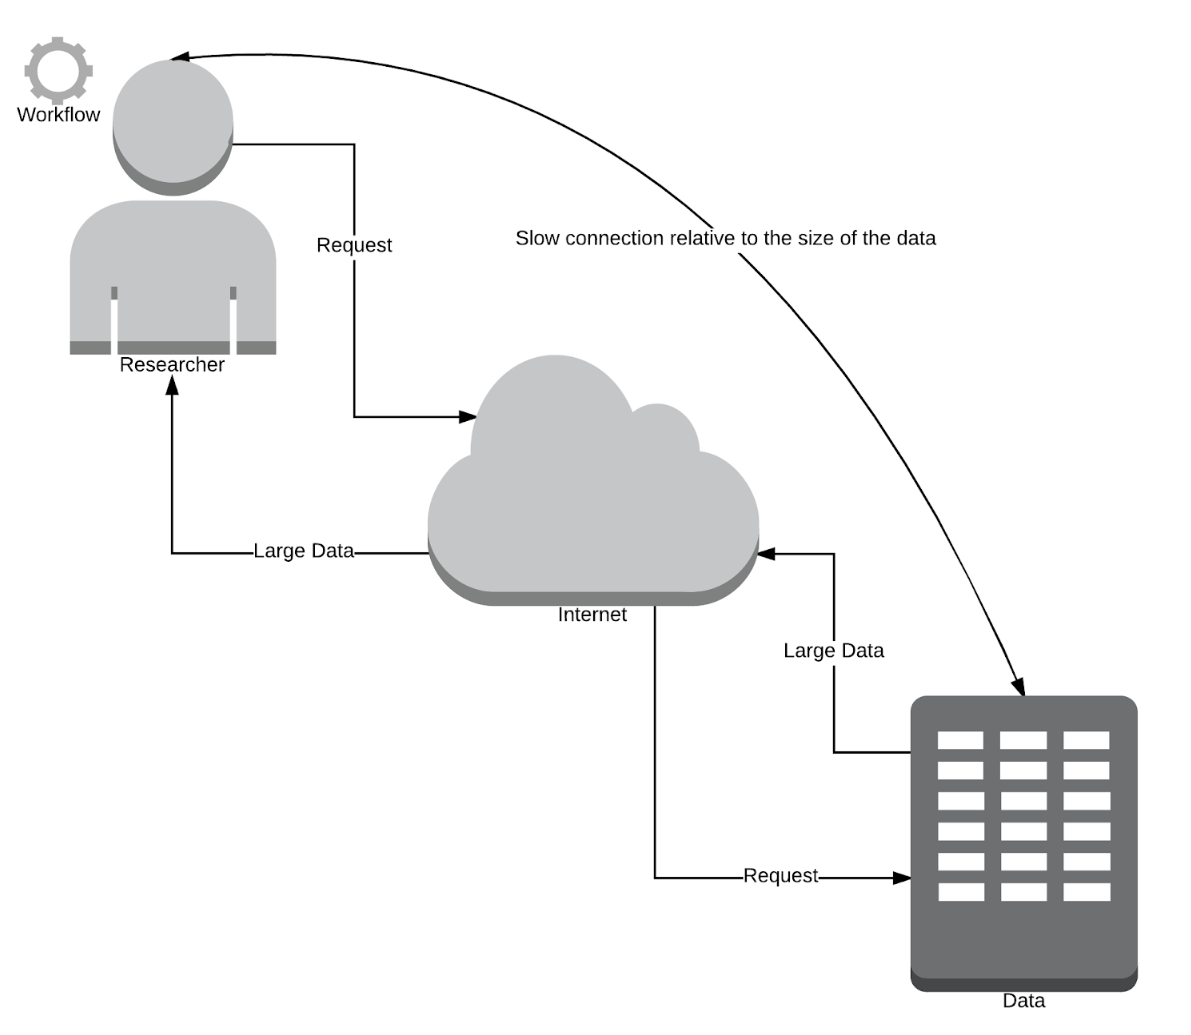
\includegraphics[width=\textwidth]{Figures/traditional_processing_model.png}
\decoRule
\caption[Traditional Researcher Data Usage Model]{This figure demonstrates how a researcher typically interacts with a remote data set. The data is transferred to the researcher via the internet in most typical environments, unless the data can be acquired through offline modes such as couriering.}
\label{fig:traditional_data_model}
\end{figure}

%----------------------------------------------------------------------------------------

Various methods for processing large data currently exist. Many of these solutions have been attempted at academic institutions such as the South African National Bioinformatics Institute at the University of the Western Cape. The next section describes some of these methods along with some advantages and disadvantages of each method.

\subsection{Traditional High Performance Computing Centers}

Processing of data at high performance computing institutions via data transfer through the use of the university network is common among research institutions where spending large amounts of money on computing resources is not a priority. Most research institutions rely on nationally available computing organisations, such as the Center for High Performance Computing (CHPC) in South Africa, to process data sets generated by their research. These organisations can be private sector businesses, government funded initiatives or a combination of the two.

HPC centres can be a viable option if the organisation offering the computing resources is not oversubscribed, has good availability and if the data set is not too large. Time may become an issue when data sets reach larger sizes, resulting in transfers that may take an unrealistic amount of time.

The CHPC is a part of the Council for Scientific and Industrial Research (CSIR)\footnote{\url{https://www.chpc.ac.za}} and provides access to two fairly powerful clusters. The main offering is the Lengau Cluster, which is a petascale system that is offered with time sharing and/or resource sharing options. They also provide access to a GPU cluster which some scientific workflow may call for.

While this has done much to aid the research tasks of various academics in the country, the CHPC is plagued with various non-user friendly issues and downtime which interfere with the researcher's deliverables.

\subsection{Inter-university Data Processing}

Universities often have very high speed networks that interconnect them nationally. In South Africa, the Tertiary Education and Research Network (TENET) of South Africa operates an internet exchange named the South African National Research and Education Network (SANReN). This network offers high speed 10 Gbps fibre channels to various universities that are involved with the project.

Researchers may be working on projects that span multiple universities. In these cases, and sometimes others, universities will provide computing resources to researchers that they are in collaboration with. The research data will either already be housed at the institution that a researcher is collaborating with or the data will need to be transferred to this university. This again could prove to be a problem if the data volumes are too large to transfer in a reasonable amount of time.

\subsection{Physically Moving Data Drives}

As previously mentioned, it is possible for data that needs to be processed to be too large to move due to reasons such as slow network speeds or data sizes that are too large. If a research institution does not have the necessary computing resources they may resort to physically moving the data that they wish to process to locations that have the ability to do so \parencite{marx2013biology}.

Utilising this method of data movement has major risks. The physical security of hard disk drives in transit can often not be guaranteed. This issue becomes compounded when the data in question is sensitive and has policies surrounding who is allowed to use it and where it is allowed to be sent.

\subsection{Utilising the Public Clouds}

Modern cloud computing offers a wide range of tools for end users to create environments to suit their needs. By offering various solutions such as Infrastructure as a Service (IaaS), Platform as a Service (PaaS) and Software as a Service (SaaS) research institutions can choose a model for data processing that fits well into their budgets. Often, a plan is chosen that allows an institution to have a chunk of storage, such as Amazon's S3, provided by the cloud provider. Data must be transferred to the cloud storage solution, after which it will be accessible from virtual machines that are created on the cloud.

This solution makes the management of hardware resources significantly easier for institutions, due to no physical hardware being owned. It also often provides more flexible computing resources as CPU, memory and disk can easily be scaled up at an additional cost with most providers.

Utilising this approach can lead to increased issues with network related activities if data volumes are large. This is mostly due to the outbound internet connection that is available in the country. The SANReN network provides a significantly faster connection locally between universities than internationally. Since most well-established cloud providers keep their data centers outside of Africa\footnote{This is true at the time of writing, but it has become evident that more cloud providers are interested in providing computing and storage resources located in South Africa \parencite{aws_sa,azure_sa}.}, the time taken to send raw data will increase substantially.

Ignoring the issues mentioned above, one major impairment to the use of cloud computing is the lack of scientific software and tools that work natively with these environments. Many scientific applications do novel operations which need to be individually catered for \parencite{barga2011bioinformatics}.

\subsection{Local Computational Ability}

Research centers, such as SANBI, may offer a local storage and compute cluster that can be used to process research data. This would be the ideal solution for most research institutions in terms of data transfer as it reduces potential problems with politics and policies surrounding certain types of data and allows quick feedback and local support. However, this requires that institutions have a large initial capital in order to purchase all the equipment needed. Once the initial setup is complete, additional expense goes towards the maintenance of the cluster as well as paying the salary of a technical officer to oversee the operation and maintenance of said cluster.

% New approaches are being attempted in order to simplify the processing of data while reducing the need to move it. This would appear to be a good solution to the issue of growing data volumes if each institution possessed the compute ability to process it all. Due to this, the next logical question to ask is whether processing can be done at the location of the data, rather than to move it before hand. This has prompted the creation of various solutions, one of which is mentioned below:

\subsection{Semi-Private Research Clouds}

Formerly known as the African Research Cloud (ARC), the South African Data Intensive Research Cloud is an inter-university research cloud project. The goal of this project is to bring storage and compute needs to Southern Africa (as well as Africa) as a whole, with each university providing parts of these services. The end user, or researcher, will be provided with a singular cloud interface with which they can create virtual compute instances and utilise data or provide their own, where the system would be intelligent enough to ensure the user is provided the resources from the centre closest to the data. The primary focus of this initiative is to support astronomy and bioinformatics workflows.

There are other project like this which aim to provide researchers in various regions and fields with flexible compute capabilities without requiring the funding to purchase and maintain physical infrastructure or make use of the more limiting HPC centers. These include the UK based Cloud Infrastructure for Microbial Bioinformatics (CLIMB) system \parencite{connor2016climb} and the Australian based National eResearch Collaboration Tools and Resources (NeCTAR) research cloud \parencite{nectar_cloud}.

\subsection{Tool Wrappers and Workflow Generators}

Projects such as the Galaxy platform introduce a visual web-based platform and extensive framework for bioinformaticists to work with tools in the field \parencite{afgan2016galaxy}. It aims to provide a way to string tools together into workflows by having tool definitions written for each piece of software and then manipulating their inputs and outputs in the context of other tools from a web interface.

It is a collaborative effort between the group that make the core service as well as the community that build the integration for it with the tools that bioinformatics researchers typically use. This approach not only allows easier consumption of larger sets of data, but also fundamentally encourages the sharing of analysis. The caveat with Galaxy is that the end-user, the researcher or academic, is restricted to using the toolset that is provided with that instance of Galaxy, whether that be the public Galaxy instances such as \url{https://usegalaxy.org}, or a Galaxy instance that is available at the researcher's institution. Software can be added, but it is a similar process to maintaining software in the traditional cluster computing way.

The Galaxy project is actively developing technology that allows this platform to sit on top of cloud environments in order to take advantage of the flexibility that they provide. Dubbed CloudMan, the project aims to enable better usage of resources and allow the project to be run on more platforms \parencite{afgan2012cloudman}. This technology is similar to other infrastructure-as-code tools such as Terraform\footnote{\url{https://www.terraform.io/}}, but it is built with a focus on compatibility with the Galaxy project.

This project is a good example of what could be used at an institution to provide analysis tools to process data that exists at the institution, provided that the software requirements are well defined by the researchers.

%----------------------------------------------------------------------------------------

\section{Project Requirements}

With respect to the research questions posed above, this thesis presents a proof-of-concept solution in the form of Nikeza. Nikeza, meaning "give away" in isiXhosa, will be a software product that compliments an existing cloud or container provisioning and orchestration environment through a plugin system. It will act as a management add-on that is written mainly in the Python programming language, specifically Python version 3, which allows it to run on most modern computing environments and operating systems. Plug-ins will be easy to write and theoretically allow many different virtual provisioning environments to utilise Nikeza.

A web application will be provided to allow users to upload their workflow document and select data from the provider's databases. The end user will also be shown updates to how their tasks are performing and when they are complete. User generated output will be moved to specific locations so that they may be retrieved by the user afterwards.

A backend service will be responsible for translating the user input from the web interface into commands that are understood by the platform that is being used at a given institution.

\subsection{System Context}

The assumption is that an institution will already be running a cloud environment and Nikeza will interface with the existing system in order to give it commands for correct execution based on the user input.

As Figure \ref{fig:existing_provider_environment} shows, the premise is that Nikeza would sit as a service which complements an existing storage and cloud infrastructure. A web interface is presented to a user with various options regarding which data he or she needs to access in order to do processing on, the location of the output data and options to upload their own workflow blueprint to the server. Once the user has submitted this, the Nikeza system translates their workflow blueprint into commands that are understood by the existing infrastructure. The user will receive periodic updates on the process of their workflow execution.

\begin{figure}[ht!]
\centering
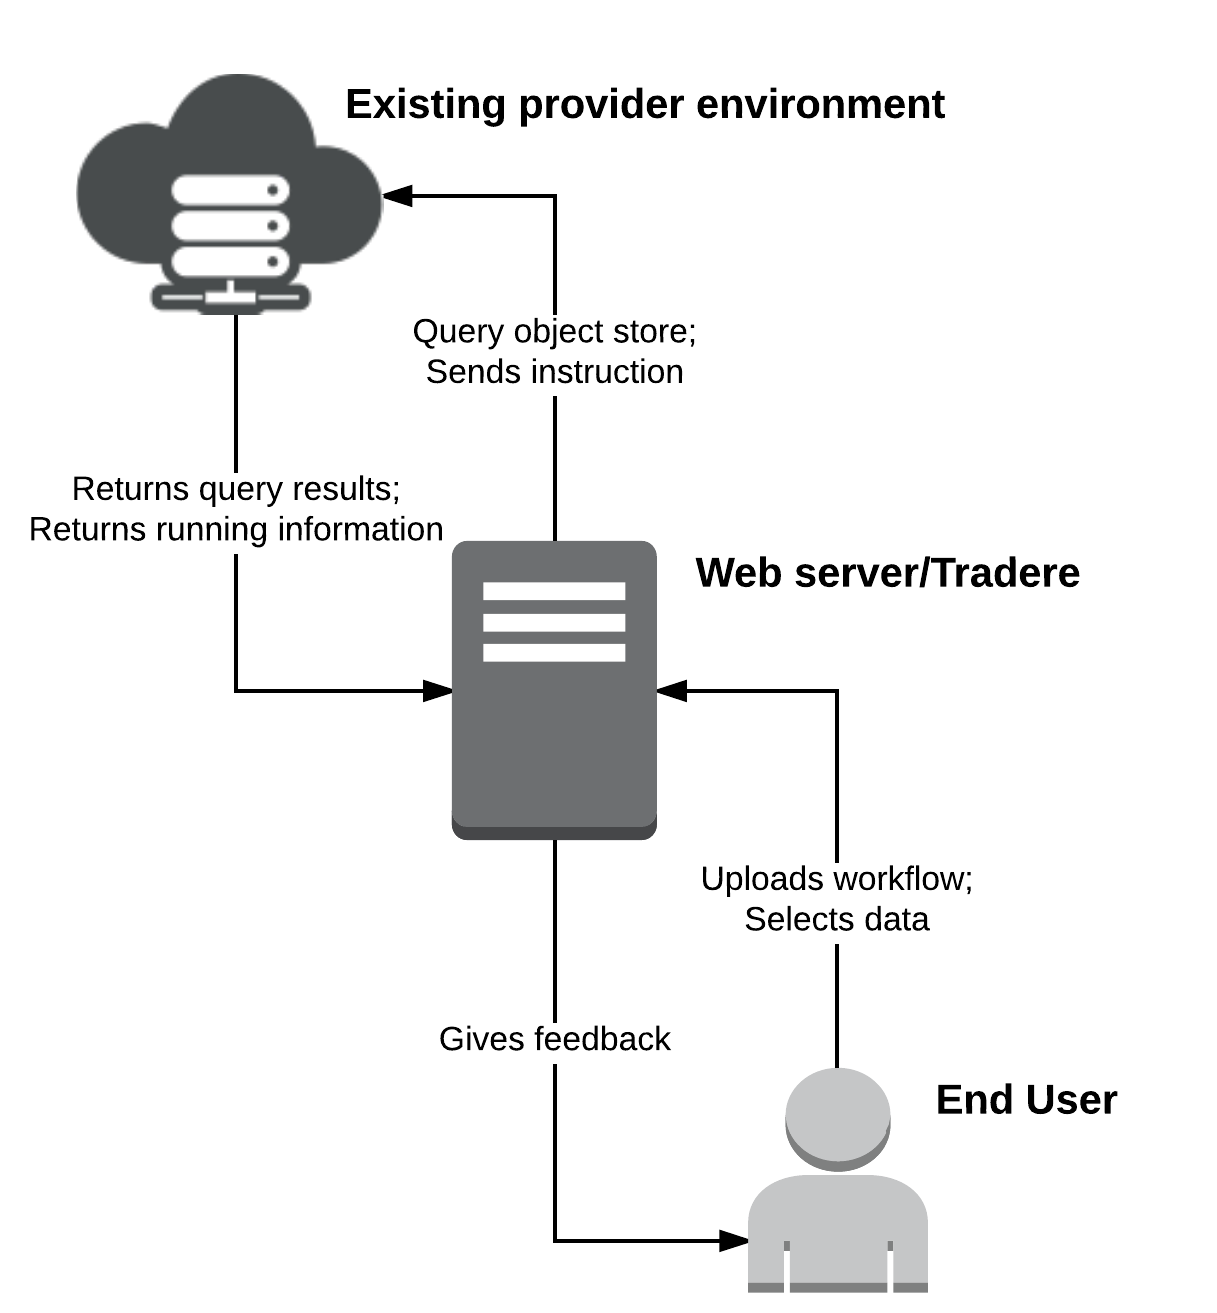
\includegraphics[width=\textwidth]{Figures/2_existing_provider_environment.png}
\decoRule
\caption[Nikeza System Context]{This figure demonstrates the concept that powers the implementation of the Nikeza project.}
\label{fig:existing_provider_environment}
\end{figure}

\subsection{Use Cases}

This section details use cases, or applications, for the proposed software system.

\subsubsection{Analysing data that is too large for a researcher to retrieve in reasonable time}

With growing data set sizes, it may not always be feasible for a researcher to wait for the retrieval of a set of data that they wish to analyse. In this case, a researcher may be able to define a workflow of the analysis that they wish to perform on data as if it were with them locally and move that definition to the environment which hosts the data. The workflow definition is understood by the remote environment and used to create a portable workflow execution environment using virtual machines and Docker containers.

Since the data already exists at the remote location, making a copy of the data set for the execution environment  or potentially, though unlikely, using it directly is objectively faster than first waiting for the data to be retrieved by the researcher. Multiple data sets may also be chained in a workflow definition, provided that all data sets exist at the remote location and are accessible to the user.

Once the execution environment completes its given objectives, the resultant data is moved off of it and onto the remote environment's storage, where the researcher is able to retrieve the completed analysis results. This could result in significantly smaller download sizes as the results of an analysis tend to be smaller than the data set itself.

\subsubsection{Sharing results of large analyses with others}

In some cases, the results of an analysis or analysis chain can be very large itself. This is seemingly counter-productive to the intended solution offered through this project. However, it is possible that collaboration efforts could lead to one researcher not actually needing to work with the results of said analysis.

In this case, one researcher would execute their analysis against a remote data set(s) and the results of that would be used by another researcher which is either closer to the data or able to execute their own analysis or analysis chain on the results of the previous.

\subsection{Conceptual Model}

The conceptual model details the components of the software architecture. This section will present the overview of the system model.

Figure \ref{fig:sytem_concept} showcases the interaction of the user and the system, as well as the various system components. This is the overview model for how the user interacts with the system and how the system responds based on the user interaction.

\begin{figure}[ht!]
\centering
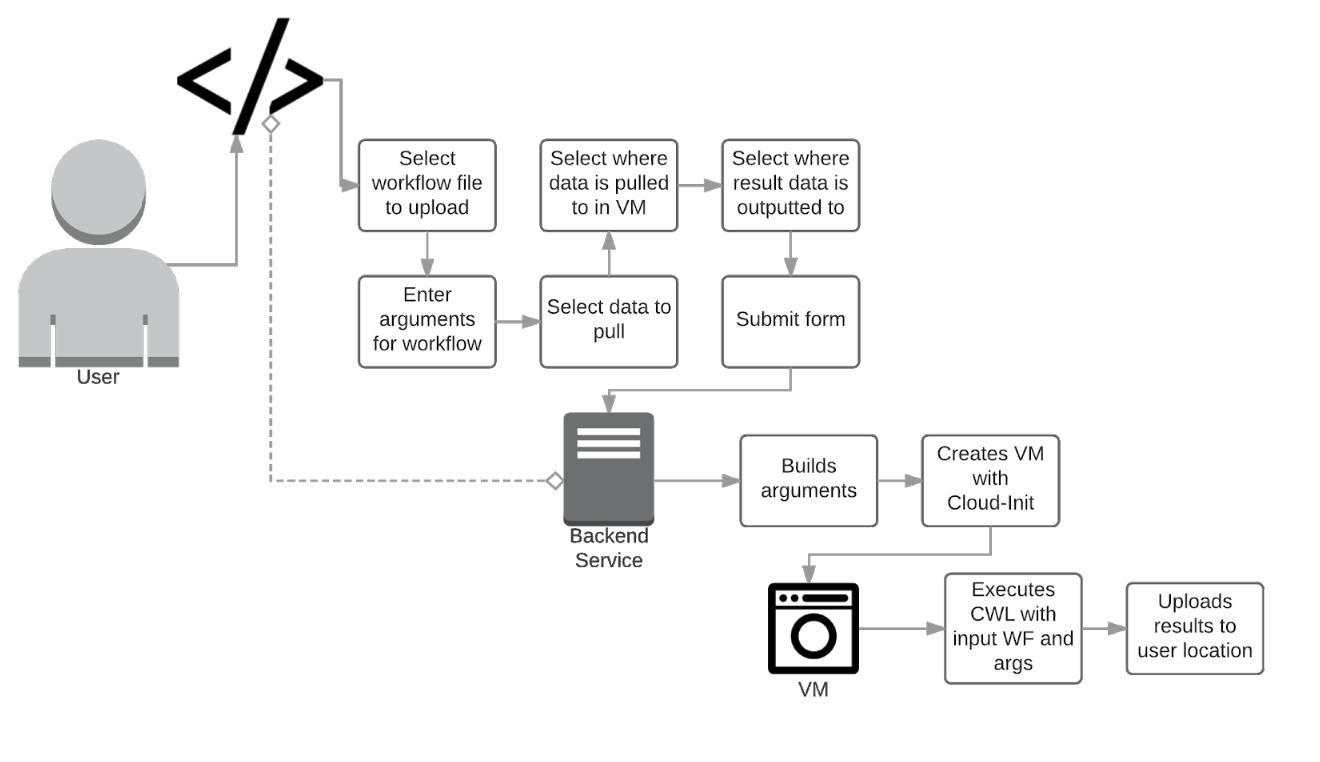
\includegraphics[width=\textwidth]{Figures/2_conceptual_model.png}
\decoRule
\caption[Nikeza System Concept]{This figure overviews the conceptual interaction model for the user and the project.}
\label{fig:sytem_concept}
\end{figure}

\subsubsection{User}

The user is able to navigate to a web interface that is provided by the project system. When first visiting this, the user is presented with a login screen so that they may authenticate against the backend system that is being used by the Nikeza system. The credentials of said user are stored with a unique cookie in the browser and on the Nikeza system side, after which they are then presented with a queue of current jobs belonging to their account. The user can select to create a new job or stop one that is already in progress. The user is also presented with a view which allows the selection of data from the backend.

\subsubsection{Nikeza System}

The project system is hosted on a public facing web server which is located near the backend cloud environment that is in use. It directly engages with the user and the cloud environment, acting as a middle man for both. The project takes care of translating user commands into instructions for the backend environment and does routine checks on jobs running for each user.

\subsubsection{Cloud Environment}

The cloud environment handles the majority of the work and takes care of running the actual analyses. It is responsible for creating virtual machines on demand, in order to accommodate the user workflow. The Nikeza system injects the workflow from the user into a newly created virtual machine and data is mapped from the storage environment into the virtual machine. Once processing is completed, the results are moved from the virtual machine into the storage environment and the virtual machine is destroyed.

\subsection{Architectural Detail}

As shown in the conceptual model (Figure \ref{fig:sytem_concept}), there are many different parts of the system that work in sequence to give the user the results. Figure \ref{fig:system_detail} expands on this and describes the complete interaction model of all the components in the system.

\begin{figure}[ht!]
\centering
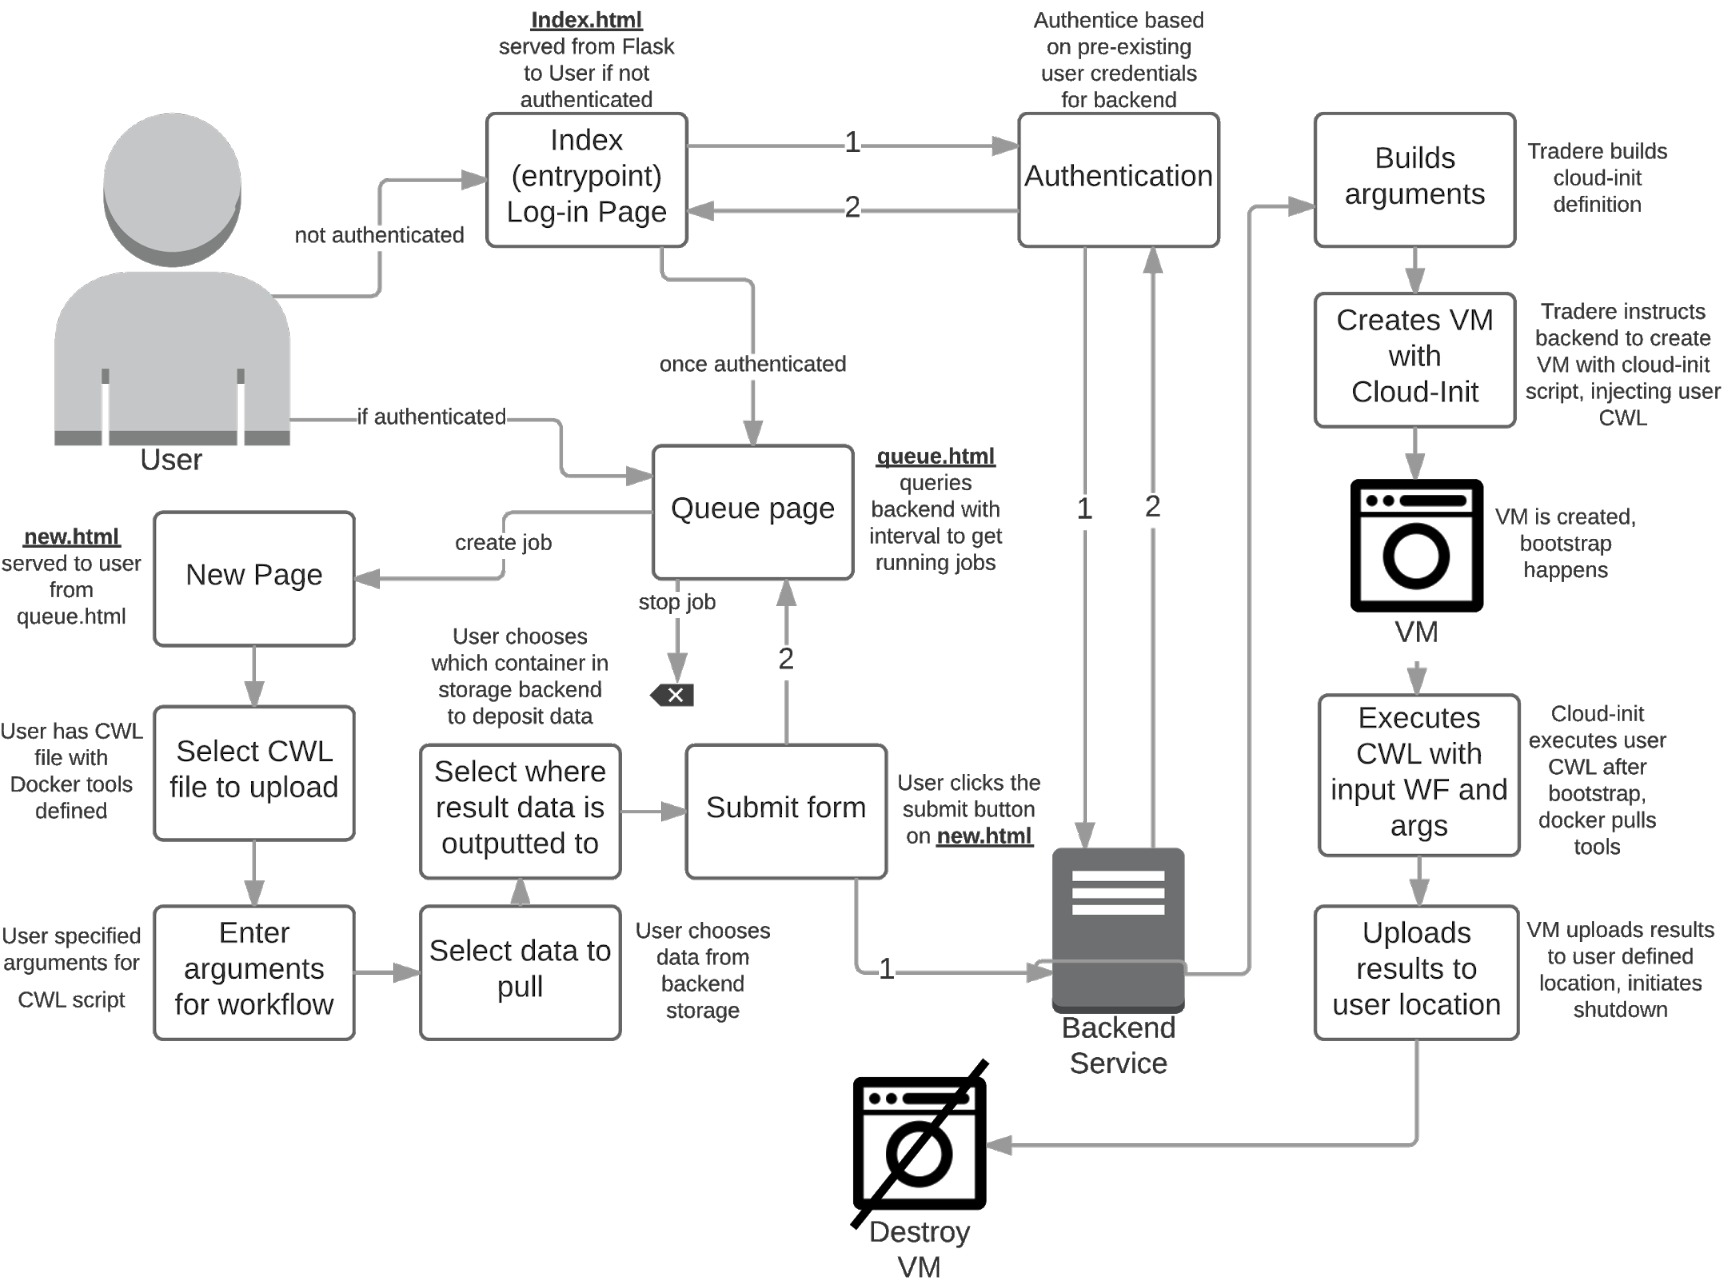
\includegraphics[width=\textwidth]{Figures/2_detailed_model.png}
\decoRule
\caption[Detailed Nikeza System Model]{This figure details the interaction model of components and the user in Nikeza. Most of the interaction behind the user-facing components are not exposed to the user and are automated.}
\label{fig:system_detail}
\end{figure}

 A new user must authenticate with the system before they can interact with it. This is done through the credentials of the cloud backend that the system is using, OpenStack in this case. The user would be provided these credentials from the institution that they want to use or from some federated authentication platform if supported. If the user has already authenticated with the system then they are not required to log in again. The Nikeza system merely tries to pass the credentials that the user supplies it through to the backend cloud environment to try to authenticate. If this fails (e.g. incorrect user credentials) then the user is presented with an error message and given the chance to try again.

The landing page for a logged-in user is the queue of jobs. This page queries the backend system for a list of jobs that may be running for that user (jobs that they have created and that are running). On this page the user can select job entries, if there are, and choose to stop the execution or they can select to create a new job. If the user selects to stop a job, an instruction is sent from the Nikeza service to the cloud platform (backend service) in order to destroy the virtual machine with the given job ID. If the user selects to create a new job they are redirected to a page that presents them with options for a new job.

The new job page will present various options for the user. These options are mandatory for submitting a new workflow and include:
\begin{itemize}
    \item Uploading their workflow definition file;
    \item Providing the arguments that the given workflow file expects when executed;
    \item Selecting the data they want to process (which is presented to them given they have access to the data through security policies/profiles);
    \item Select where the data-to-be-processed is pulled into and the resultant data is generated on the virtual machine that will be created for their workflow;
    \item Select where the resultant data is uploaded to on the backend service. 
\end{itemize}

The user can then select whether to start the job or to cancel and return to the queue without adding the new job. If the user selects to start the job, the workflow definition is uploaded from their computer and, along with all the parameters that the user filled in, an instruction log is generated by Nikeza. A virtual machine creation is requested by Nikeza and the instruction log is specified to bootstrap the creation of the virtual environment. In the meantime, the user is redirected to the queue page, where they can see the status of the virtual environment that is running their workflow. Once the job is completed in the virtual machine the data is moved to where the user specified and the virtual machine is destroyed, removing it from the queue page, and the user can retrieve the data by logging into the backend dashboard.

\subsection{Technical Functionality Requirements}

The overall goal of Nikeza is to provide an easy-to-use interface for end-users to submit their workflow to a cloud environment in which some research data is located in order for their workflow to be executed with minimal interaction. The functionality below provides the ability to answer the research questions being asked in this thesis.

\subsubsection{Allow users to execute scientific workflows without needing technical expertise}

The user's workflow submission must be understood by the system and automatically executed without leaving things behind on completion. It should be fully automated.

\subsubsection{Allowing users to execute scientific workflows on data that does not exist locally}

The user must be presented with a list of data, which they would have access to through pre-specified policies. They must be able to select the data that they want to do processing on.

\subsubsection{Allowing the system to run without modifying existing backend environments}

Nikeza must be designed in such a way as to allow the existing backend setup to stay intact, with minimal to no changes required by administrators. 

\subsubsection{Easy-to-use, human friendly user interface for the web application}

The user must be presented with an easy to understand, human friendly web interface which has all the technical details and commands abstracted.

\subsubsection{Simple plugin system in order for providers to be able to easily adapt Nikeza to their environment}

The application should support different environments through a translation plugin system in which the administrator of a system can write the needed operations in order to support their system.

\section{Testing Framework}
<!-- include stuff there -->